\documentclass{article}
\usepackage{indentfirst}
\setlength{\parindent}{2em}
\usepackage{graphicx}

\title{SYSC 5001W: Project deliverable 1} % Title of the assignment

\author{Qiguang Chu\\ \texttt{300042722}} % Author name and email address

\date{University of Ottawa --- \today} % University, school and/or department name(s) and a date

%----------------------------------------------------------------------------------------

\begin{document}

\maketitle % Print the title

\section{Problem Fomulation} % Numbered section
	A factory assembles three types of products P1, P2, and P3, in which each product needs a unique combination of gears. It totally has three components C1, C2, and C3. Product P1 includes one C1, product P2 needs one C1 and one C2, and product P3 contains one C1 and one C3.
	
	There are two inspectors to clean and repair these gears. Inspector 1 works on C1 components. Inspector 2 works on C2 and C3 randomly. 
	
	It has three workstations named W1, W2, and W3, which assemble products P1, P2, P3, respectively. Components are sent to their belongings workstation individually. 
	
	Each workstation has a buffer capacity of two components, with one buffer available for each of the component types needed. A product can begin being assembled only when components of all types required are available. If all workstation buffers for a specific type of components are full, the corresponding inspector who finished inspecting a component with the same type is considered “blocked" until there is an opening, at which time the inspector can resume processing and sending components of that type.

\section{Setting of Objectives and Overall Project Plan}

Question: Is there any way to shorten the process total time of producing specific number of products?

The criterion for evaluating effectiveness: the average delay time of each component.

We already have schedules of every component of a specific products. Once the buffer is fulfill, inspectors have to wait until the buffer is available again. 

 Resource required: 2 people for 10 days for data collection, 1 person for 5 days for data analysis, 1 person for 5 days for model building, 1 person for 3 days for running the model, 1 person for 4 days for implementation.

\section{Model Conceptualization}
\begin{figure}[htbp]
\begin{center}
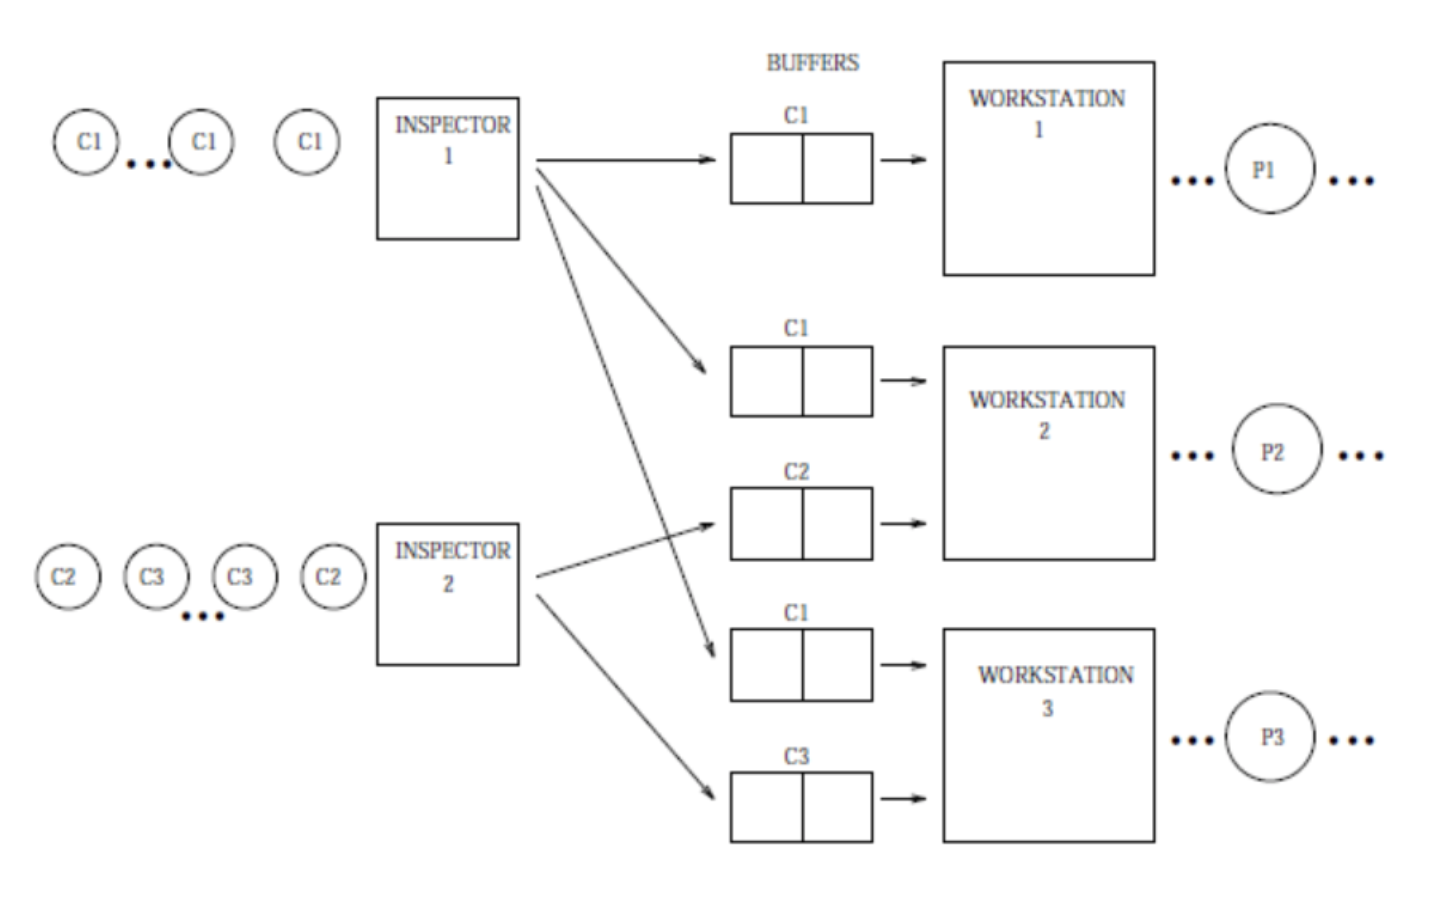
\includegraphics[width=5in]{Process.png}
\caption{Flow Chart}
\label{default}
\end{center}
\end{figure}

We have the process of producing products P1, P2 and P3. In order to simulate it correctly and specifically, The model and its attributes and relative relations have to be conceptualized. 

\subsection{Entities}
\subsubsection{Component}

Component is the main element we consider in this model. The attribute of components are quite simple because they only use labels to differentiate them. I have to say each component is a part of a production. Here we have C1, C2 and C3. The support of components are consistently.

\subsubsection{Inspector}

We totally have two inspectors, Inspector 1 and Inspector. Each inspector can inspect component it receives. But there's a little difference that Inspector I only deal with Component 1 while Inspector 2 deals both C2 and C3. The main activity of a inspector is to deal with components and send them to specific workstations.

\subsubsection{Workstation}

Workstations are places to operate components and output products. We have three workstation totally, Workstation 1, Workstation 2 and Workstation 3. Workstation1 only need one C1 gear to produce a P1 product. Workstation 2 requires C1 and C3 while Workstation 3 asks for C1 and C3. Each workstation also has a buffer, which has two room for each kind of coming components. For each production it needs some time to operate.

\subsubsection{Product}

We have three kinds of products, Product 1, Product 2 and Product 3. Each product is produced by its correspondingly workstation. 

\subsection{Attributes}

\begin{enumerate}
\item Component: Classification
\item Inspector: Number, Dealing time, Work condition
\item Workstation: Number, Operation time, Buffer, Work condition
\item Production: Classification, Ingredient
\end{enumerate}

\subsection{Event}

\begin{enumerate}
\item Inspector sends a component to a workstation.
\item A workstation finished an operation on a product and output

\end{enumerate}

\subsection{Activity}
\begin{enumerate}
\item Inspection time of a component
\item Operation time of a product
\end{enumerate}

\subsection{Interaction}

\subsubsection{Components and Inspectors}
Inspectors spend time on dealing with components and then send them to workstations.
\subsubsection{Components and workstations}
Workstations spend time on operation on components and output them
\subsubsection{Components and product}
Products are assembled from specific components.
\subsubsection{Inspectors and workstations}
Inspectors send specific components to specific workstations. Inspector will consider the optimized method to send them right way. If the buffer of a workstation of one component is fulfill, then the inspector may be blocked and have to wait the available of that buffer to keep working.
\subsubsection{Products and workstations}
Each workstation produces a specific product.


\section{Model translation}
\begin{figure}[htbp]
\begin{center}
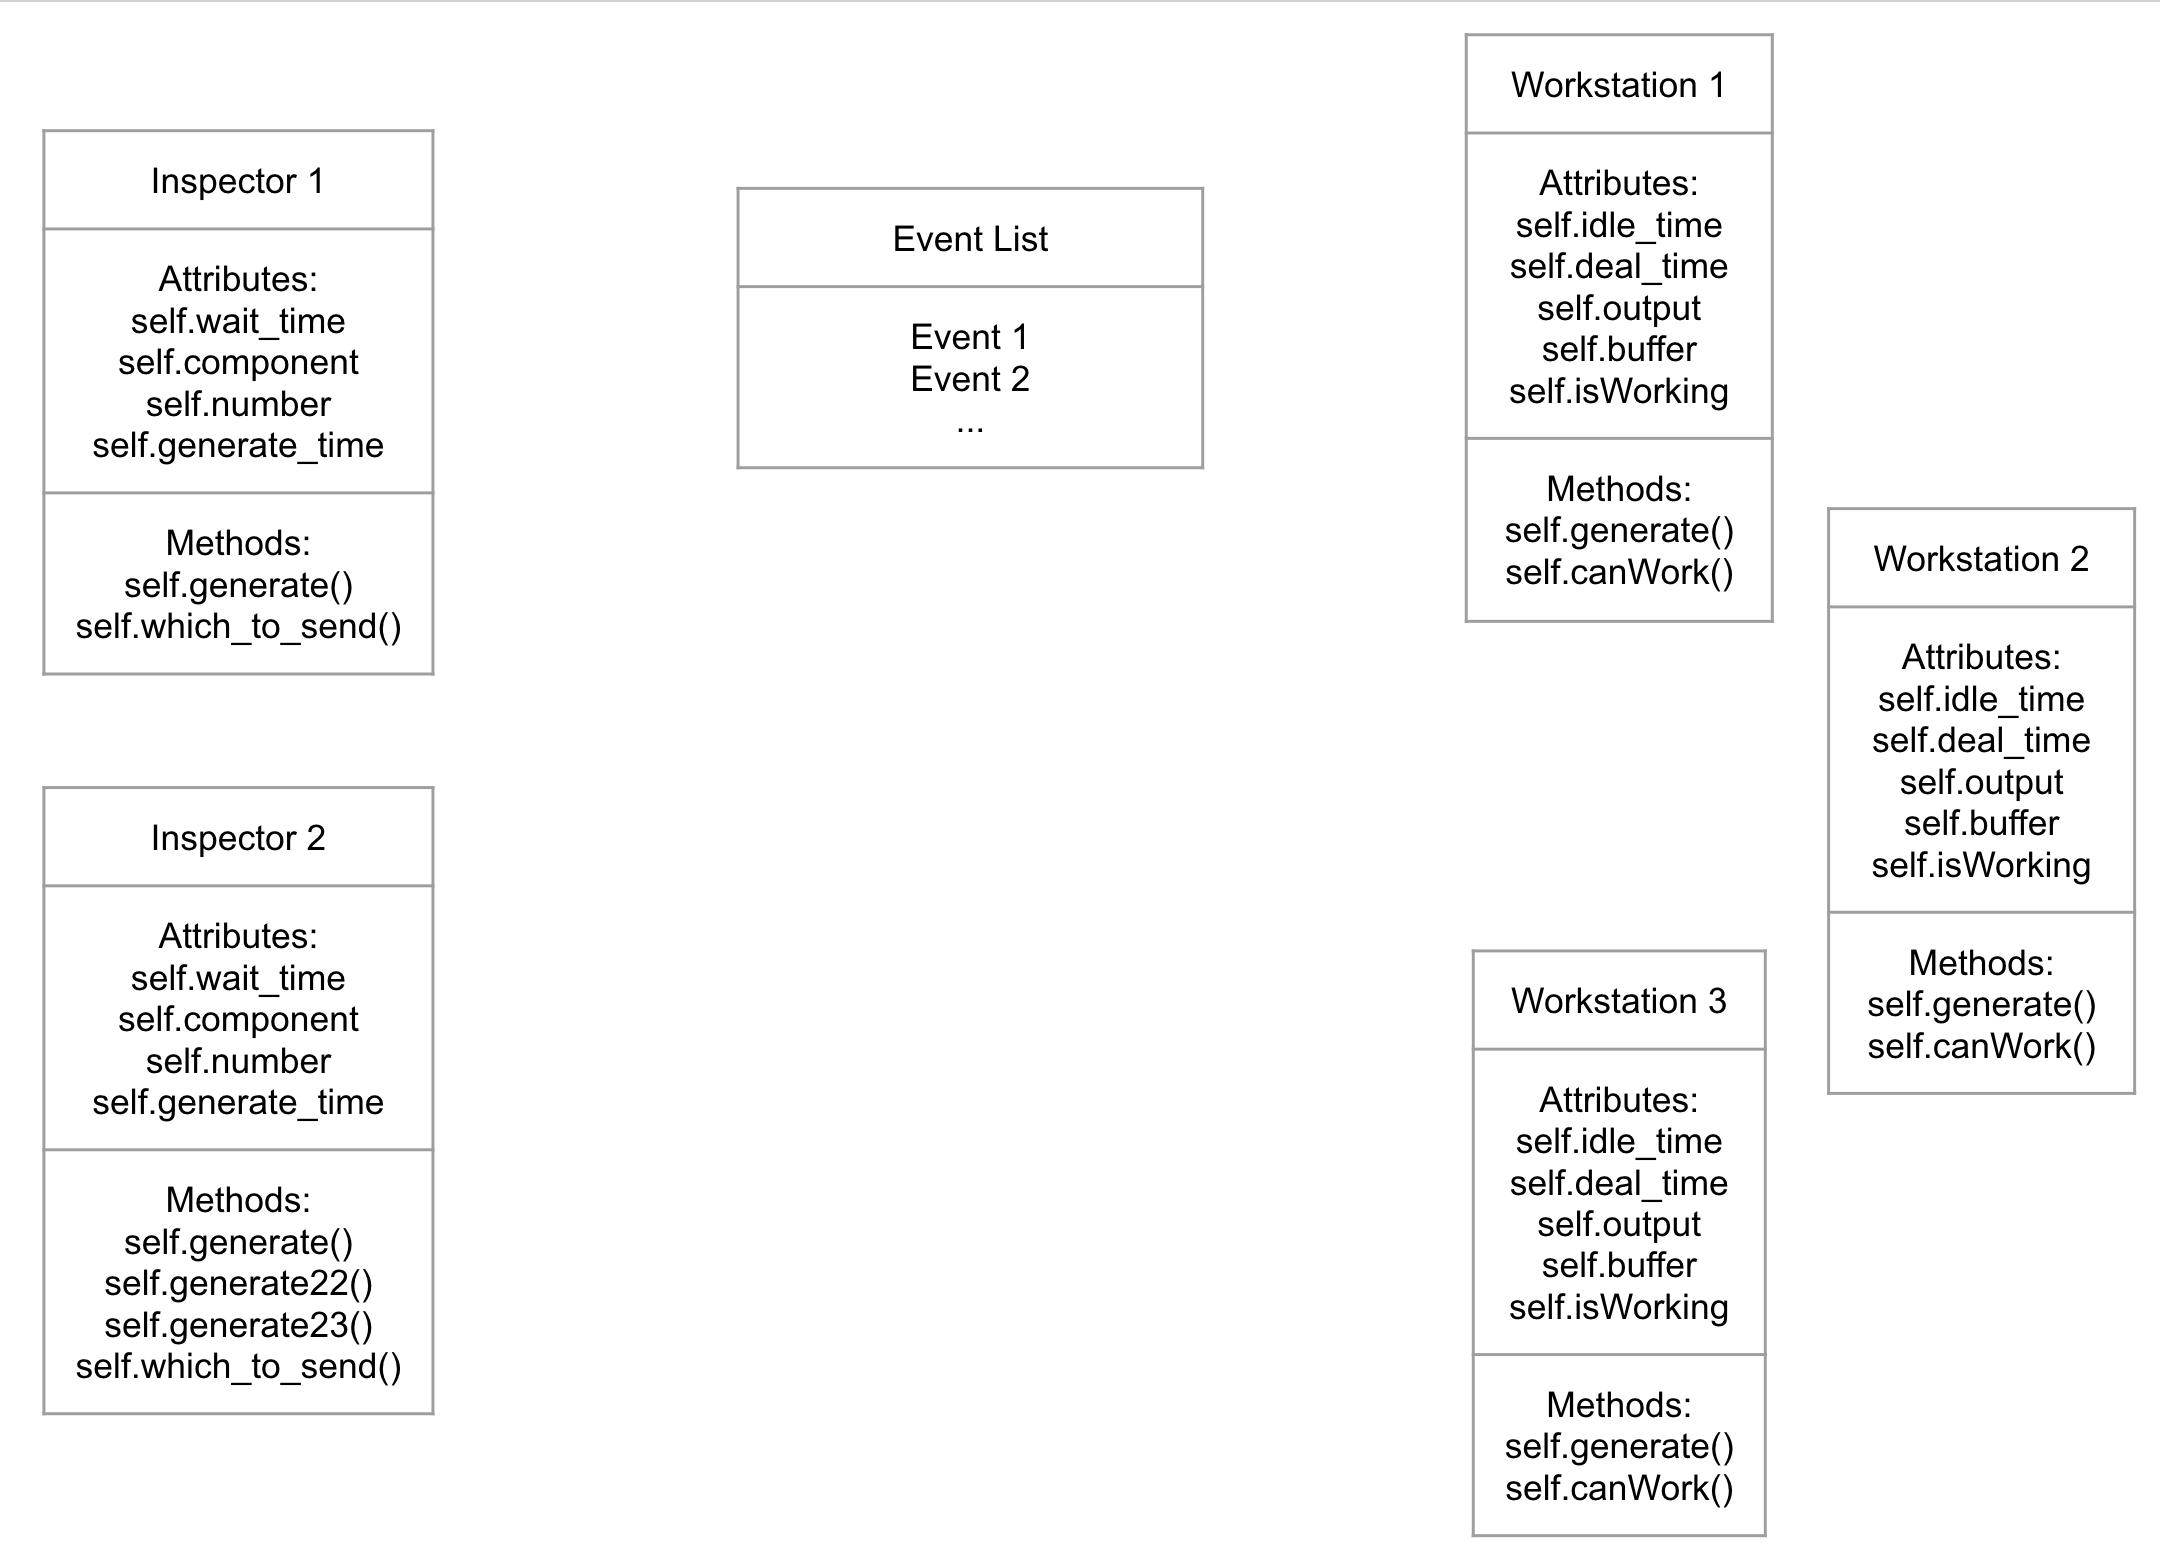
\includegraphics[width=5in]{Architecture.png}
\caption{Model architecture}
\label{default}
\end{center}
\end{figure}
\subsection{Modeling Language}

I choose Python as the main modeling language of this process. Python is a simple high level language and it's more convenient to use for objective oriented programming. The software I use is Pycharm, which is a great IDE client of Python.

Python is easy to read and maintain, and the processing speed is faster than R, without cutting the database;

Python has a strong momentum, many large companies need it, and the market has a bright future. However, MATLAB language is relatively limited, focusing on engineering and scientific computing. Python has a rich extension library

\subsection{High level description}

\subsubsection{FEL}
The simulation starts from a future event list(FEL), which has Inspector1 and Inspector2 to deal with and the simulation terminates with nothing in the FEL. For each step, we sort the FEL to find the nearest event to occur and take it out. The finishing of one event may triggers other events to happen and we add them all to FEL. The primary key of the event list should be the clock, which I note as Worldtime in the code. The clock has to be sequenced for every loop in the circle. Then it comes to the subjective of this event, which can be Workstation1, Workstation2 or Workstation3. After that, the component being transferred will be the next element like Component1, Component2 or Component3. The last element would be two activities, 'receive' and 'output'. 'receive' means that a workstation receives a component from a inspector, while 'output' denotes that a workstation outputs a product.

\subsubsection{Block}

There is one case that an inspector may be blocked when the corresponding buffer of the specific workstation is full. For example, Inspector1 plans to send Component1 to Workstation1 but there already exist two C1 in the buffer of Workstation1(Workstation1 only has one buffer and that is for C1). The transfer of Inspector1 is blocked and it cannot keep inspecting other components. It has to wait for the output of that workstation so the buffer would minus one or wait for the other component needed for the product in this workstation and thus the workstation can operate.

\subsubsection{Idle}

Correspondingly, in short supply, workstations may face that no work to do. That is because the workstation does not have necessary gears. If we want the total time to be shorten, we have to get rid of this situation as much as possible. The calculation of idle time of the workstation would be the start time of working minus the time of the last finished operation.























\end{document}